\documentclass[12px]{article}
\usepackage{vub, pgfplots, amsmath, amsthm, amssymb, graphicx, float, placeins, makecell, subcaption, caption}
\usepackage[utf8]{inputenc}
\usepackage[T1]{fontenc}
\usepackage[backend=biber]{biblatex}
\pgfplotsset{compat=1.16}
\graphicspath{ {./images/} }

\renewcommand{\figurename}{Figuur}
\renewcommand\theadfont{\bfseries}
\renewcommand\theadalign{bl}

\title{Databanken en webtechnologie}
\subtitle{webapplicatie}
\author{Partous Pieter}
\faculty{Industrieel ingenieur}


\begin{document}
\maketitle
\begin{abstract}
In dit verslag geven we een korte overzicht van wat er in de webapplicatie te beleven valt. Ondere andere het model van de databank en een beschrijving van enkele fautures die terug te vinden zijn op de webpagina's.
\end{abstract}

\section{Databank model}
Op figuur \ref{graph1} kan je de structuur van de databank terug vinden. De tabellen 'movie\_reception' en 'comments' staan wel in de databank maar werden verder niet toegepast in de webapplicatie, al de andere tabellen worden wel gebruikt.
\begin{figure}[!hbp]
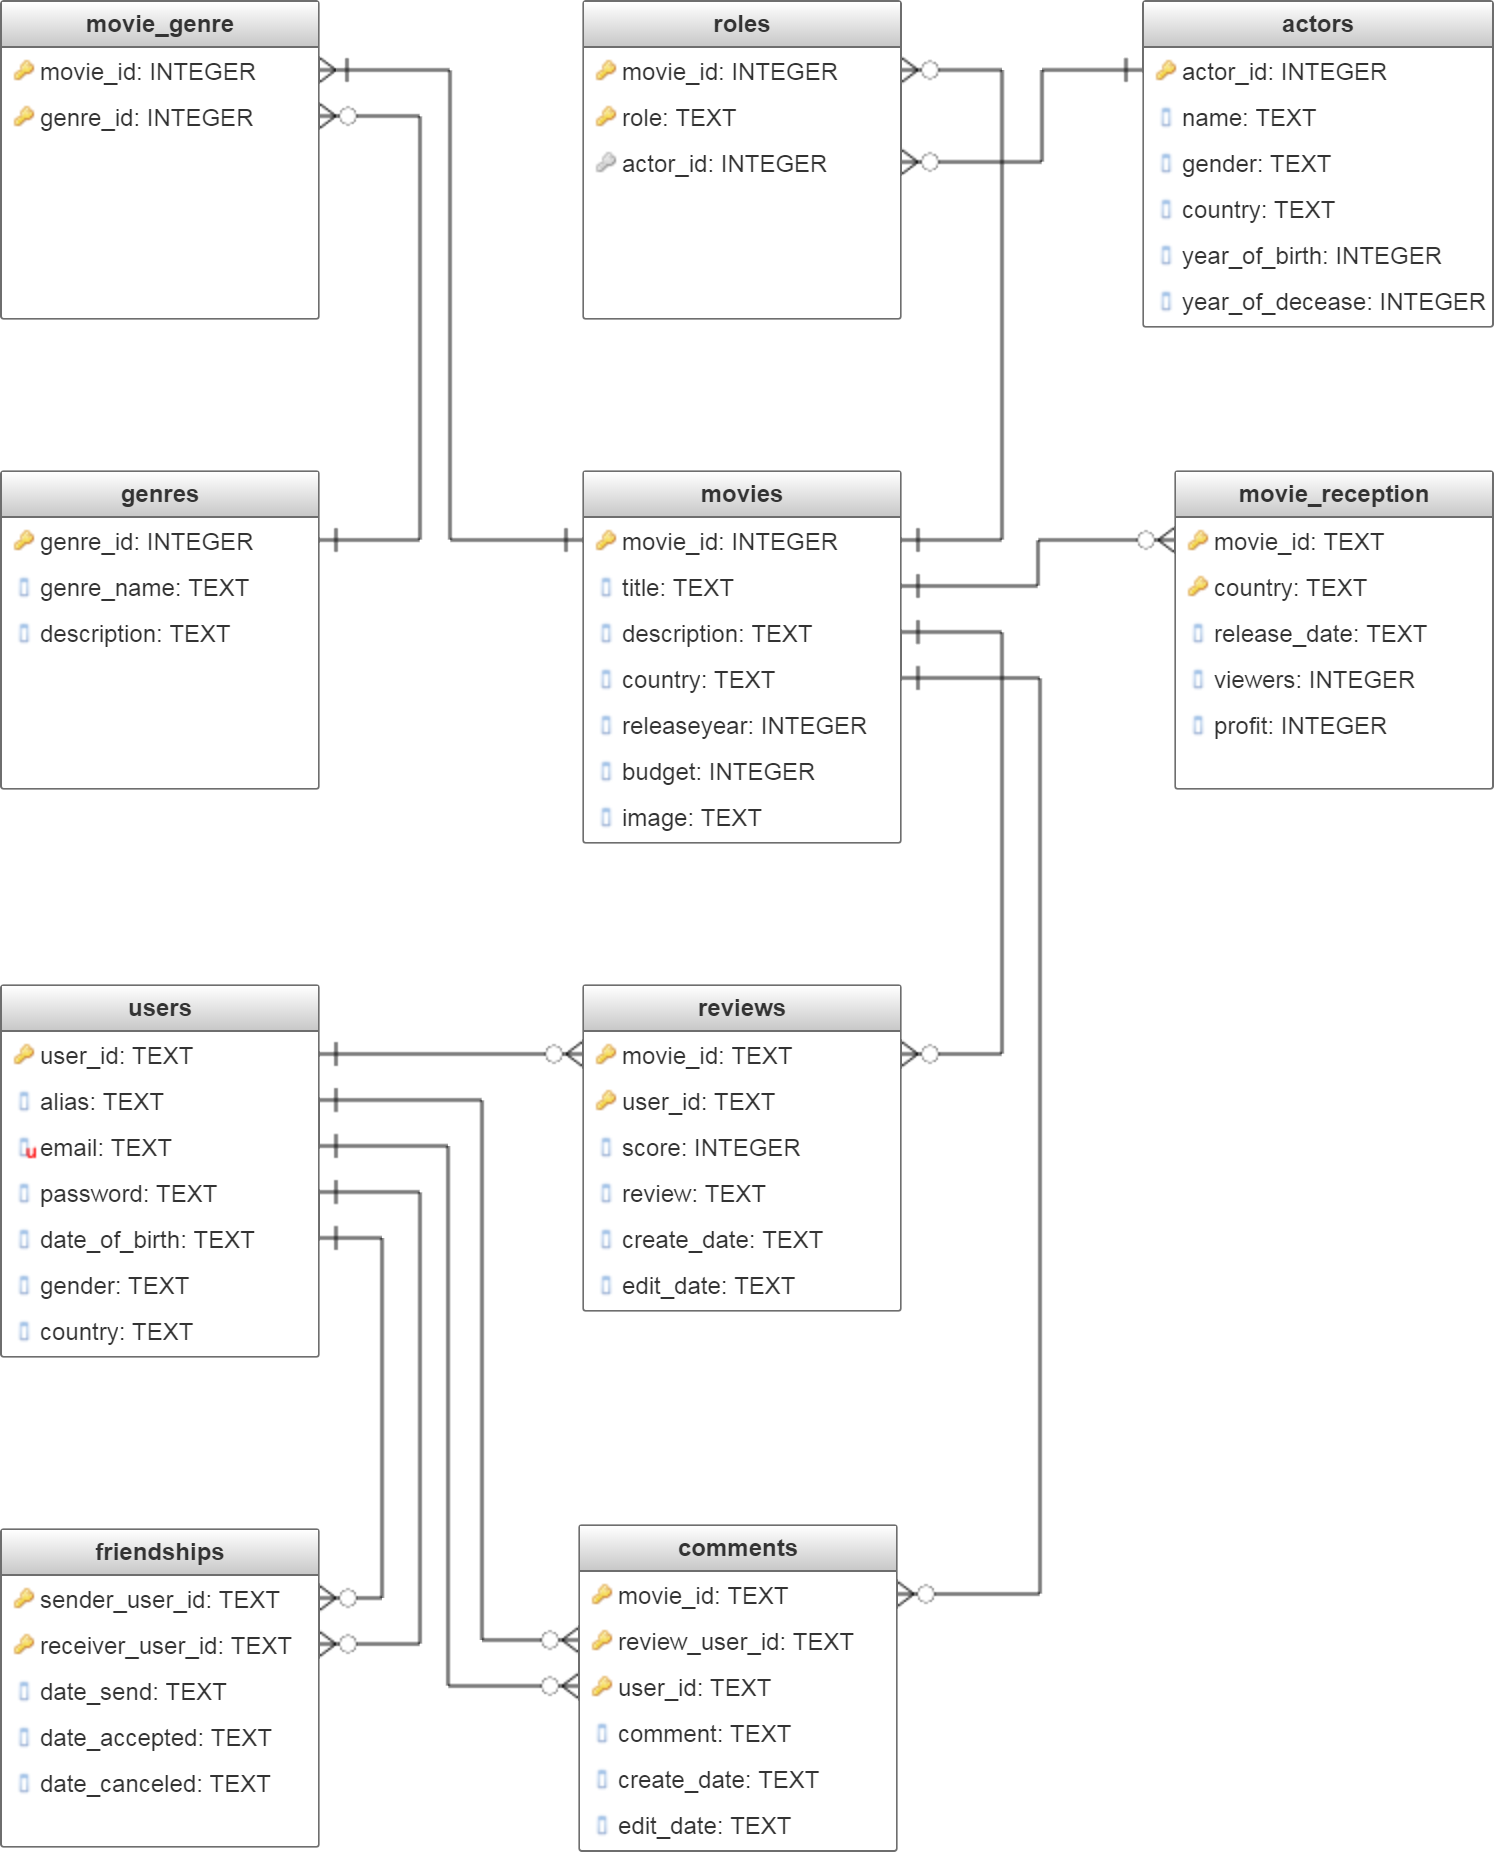
\includegraphics[width=\textwidth]{database-graph}
\caption{Database structuur.}
\label{graph1}
\end{figure}
\FloatBarrier

\section{Extra packages}
Om er voor te zorgen dat de webapplicatie gemakkelijk te stijlen is heb ik gebruik gemaakt van Bootstrap (https://getbootstrap.com/). Dit is een bibliotheek met een hoop vooraf gemaakte css classen en JavaScript hooks. Verder is er ook gebruikt gemaakt van JQuery (https://jquery.com/) om de zelf geschreven JavaScript eenvoudiger te maken en van Sass (https://sass-lang.com/) welke een css preprocessor is  en het mogelijk maakt om functies, mixins en nesting toe te passen. De sass bestanden (.scss) worden daarna omgezet in zuivere css bestanden met behulp van Node.js (https://nodejs.org/en/). Het script dat de omzetting doet kan terug gevonden worden in het bestand 'gulpfile.js'. vooraleer het script in de gulpfile kan uitgevoerd worden moeten eerst de nodige node packaged geinstalleerd worden, dit kan gedaan worden door 'npm install' in de command line uit te voeren in de root van het project.

\section{Homepage}
De link '/' wordt automatisch omgeleid naar de link '/Homepage'. Op deze pagina kunnen we zoeken naar filmen door de filteren op titel en genre. Hier zijn ook twee extra knoppen toegevoegd die door middel van JavaScript alle genres kunnen selecteren/deselecteren.
\begin{figure}[!hbp]
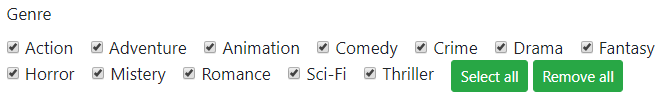
\includegraphics[width=\textwidth]{genre-select}
\caption{Genre selectie.}
\end{figure}

\section{Movie details}
Op de hoofdpagina heeft elke gevonden film een knop 'View details', deze brengt ons naar de pagina '/Movie deatails/<int:movie\_id>'. Op deze pagina kunnen we de details van de film zien alsook enkele rollen en acteurs die in de film meegespeeld hebben. Onderaan de pagina kunnen we een review schrijven en een rating aan de film geven. Elke gebruiker kan slechts één review schijven en indien ze al een review hebben dan hebben zij de optie om hun review terug te verwijderen. De gebruiker moet uiteraard ingelogd zijn om een review te schrijven en als dit niet het geval is dan verwijst de 'Add review' knop naar de login pagina.

Rechts vanboven op de pagina is er ook een knop 'Edit' die naar de bewerkings pagina leidt.
\begin{figure}[!hbp]
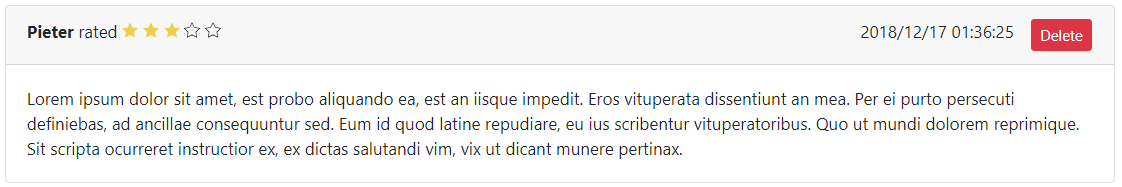
\includegraphics[width=\textwidth]{review}
\caption{Voorbeeld van een review.}
\end{figure}
\FloatBarrier

\section{Edit movie details}
Om toegang tot deze pagina te krijgen moet men ingelogd zijn. Hier kan men dan de details van de film aanpassen alsook rollen en acteurs toevoegen of aanpassen. Voor de rollen is er zelf geschreven JavaScript gebruikt om gemakkelijk meer rollen toe te voegen of te verwijderen. De meeste velden hebben ook een 'required' atribuut waardoor ze dus niet leeg door verzonden kunnen worden.

Dezelfde pagina is gebruikt als men op de 'Add movie' knop drukt in de header van de site. In dit geval zullen al de velden gewoon nog blank zijn.

\section{Login/register}
Als er op de knop 'Log in' in de header van de pagina geklikt wordt of indien er een actie word uitgevoerd waarvoor de gebruiker ingelogd moet zijn worden we verwijst naar de login pagina. Hier kan men inloggen of registreren. Bij het registreren wordt er gecontroleerd of de twee ingevoerde paswoorden gelijk zijn aan elkaar vooraleer het verzoek verzonden wordt naar de server.
\begin{figure}[!hbp]
\centering
\begin{subfigure}{.5\textwidth}
	\centering
	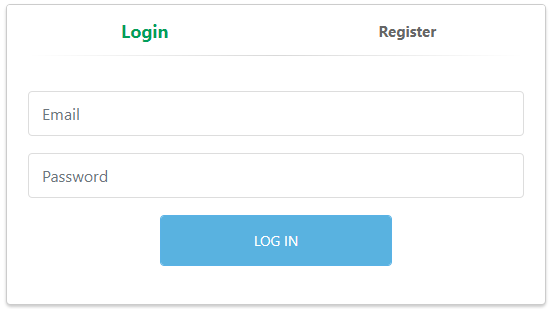
\includegraphics[width=.8\textwidth]{login}
\end{subfigure}%
\begin{subfigure}{.5\textwidth}
	\centering
	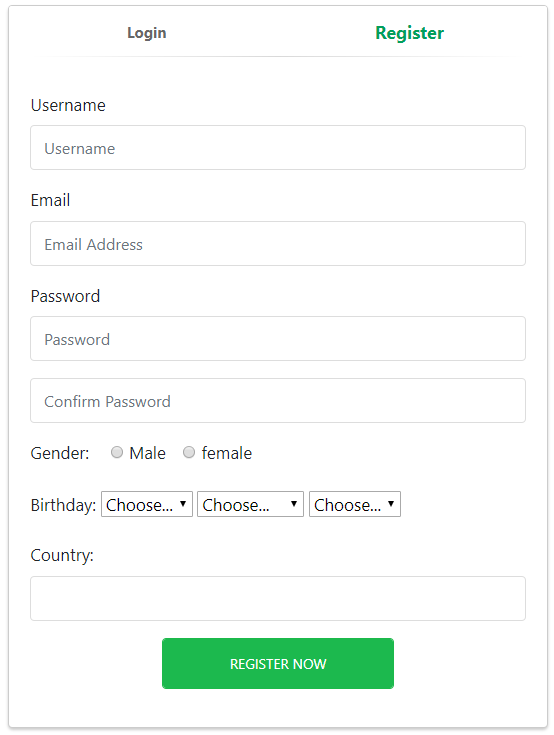
\includegraphics[width=.8\textwidth]{register}
\end{subfigure}
\caption{Login en resister forms.}
\end{figure}
\FloatBarrier

\newpage
\section{Add friends}
In de header van de pagina is er een knop 'Add friends'. Hier kan er gezocht worden naar gebruikers door te filteren op alias. Voor al de gevonden gebruikers kan er een vriendschaps verzoek verzonden worden.
\begin{figure}[!h]
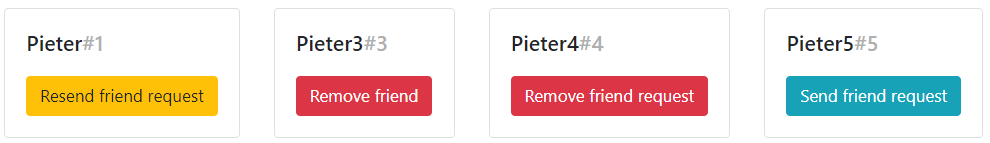
\includegraphics[width=\textwidth]{user-search}
\caption{De knoppen hebben een verschillende text afhankelijk van de huidige toestand van het verzoek.}
\end{figure}
\FloatBarrier

\section{User page}
Indien ingelogd kan men op de gebruikers pagina komen door op naam te drukken links van de 'log out' knop. Op deze pagina kan men vrienden en vriendschaps verzoeken zien, accepteren en verwijderen. Indien men naar een userpage van een andere persoon probeert te gaan zal er een forbidden access error getoont worden.
\begin{figure}[!hbp]
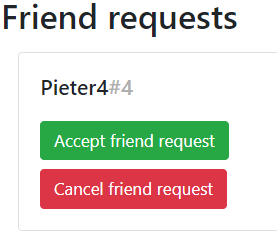
\includegraphics[width=.3\textwidth]{vriendschapsverzoek}
\centering
\caption{Een vriendschaps verzoek aanvaarden of negeren.}
\end{figure}
\FloatBarrier

\section{Besluit}
Met dit project heb ik een hoop bijgeleerd over hou SQL werkt en gebruikt wordt. Ik ben ook verbeterd met het gebruik van python sinds ik hier nog niet veel mee gewerkt had. Ik moet wel toegeven dat dit project meer werk vroeg dan ik verwacht had waardoor er enkele functies zijn die ik oorspronkelijk had willen toevoegen maar waar ik geen tijd meer voor had. 


\end{document}
